\chapter[Introduction]{Statistics in the modern day}\label{intro}


The goal of statistical analysis is to use data to estimate and test
the parameters of a model.

Figure \ref{modelflow} shows a model in flowchart form.  Data and
parameters are fed into a function, and the function spits out some
output. We then evaluate the output based on some criterion, typically
regarding how well it matches some portion of the data. Our
goal is to find those parameters that produce output that best meets
our evaluation criterion.


\begin{figure}[htb]
%\hskip -1.4cm
\begin{center}
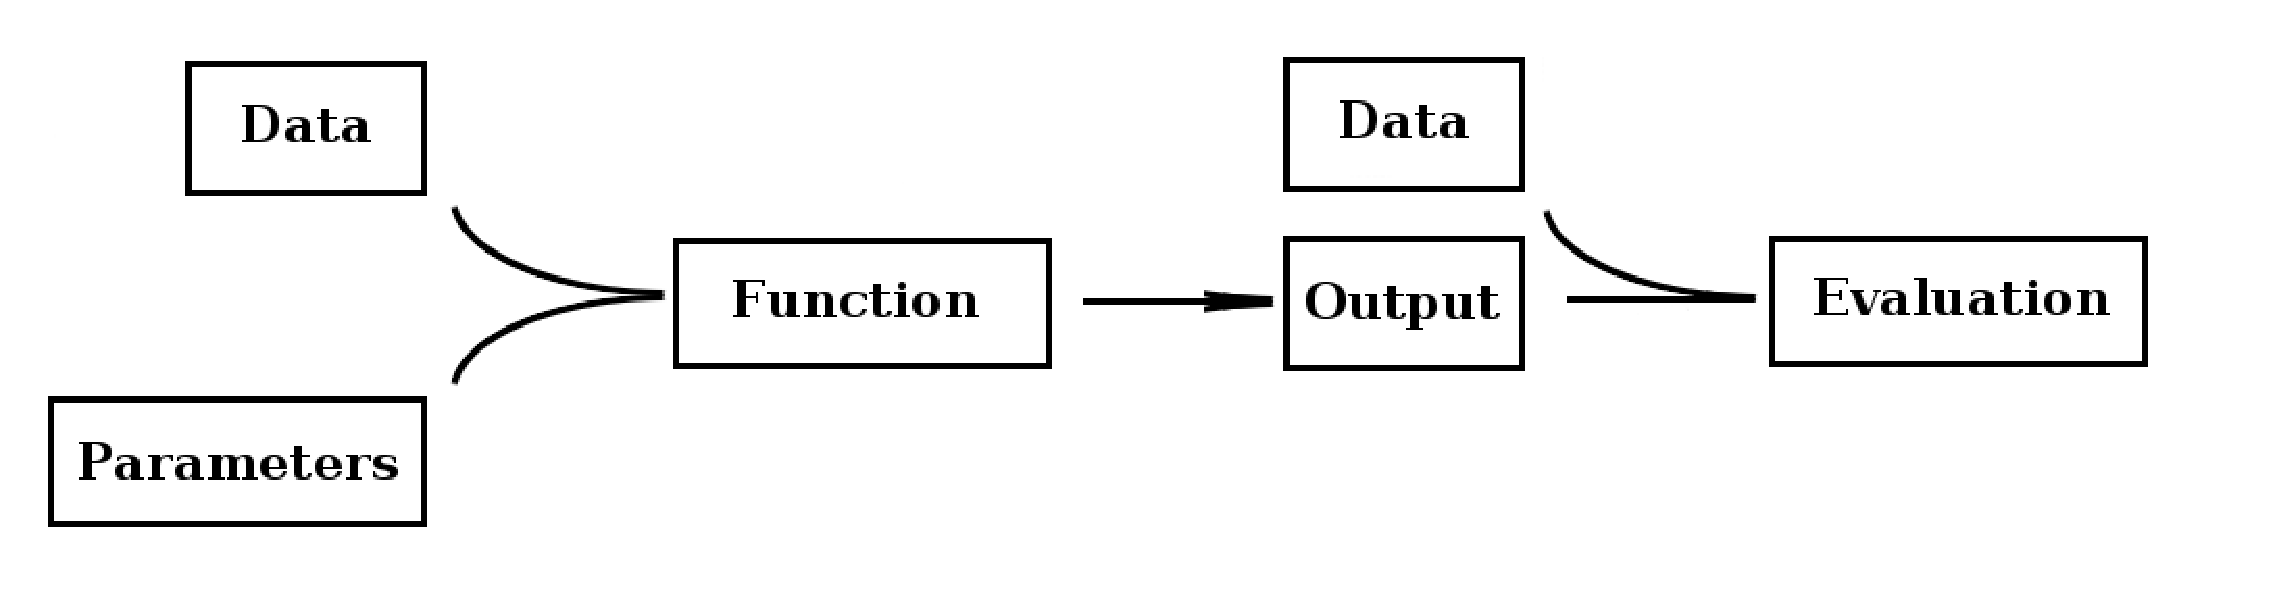
\includegraphics[width=\textwidth*\real{1.05}]{models}
\end{center}
\caption{A flowchart for distribution fitting, linear regression,
likelihood functions, multilevel modeling,
simulation (including agent-based modeling), data mining, non-parametric modeling,
and various other methods.}
\label{modelflow}
\end{figure}

One example is the \ind{Ordinary Least Squares} model. Let $\Xv$
indicate the independent data, $\betav$ the parameters, and $\yv$ the
dependent data. Then the function box consists of the simple equation
$\yv_{\rm out} = \Xv\betav$, and the evaluation step seeks to minimize
$(\yv_{\rm out} - \yv)^2$. 

For a simulation, the function box may be a complex flowchart in which
variables are combined nonlinearly with parameters, then feed back upon
each other in unpredictable ways. The final step
would evaluate how well the simulation output corresponds to the
real-world phenomenon to be explained.

The problem of statistical modeling is to find the parameters at the
beginning of the flowchart that will output the best evaluation at the
end. That is, for a given function and evaluation in Figure
\ref{modelflow}, we seek a routine to take in data and produces the optimal parameters, as in Figure \ref{modelflowback}.
In the OLS model above, there is a closed-form solution to the problem:
$\betav_{\rm best}=(\Xv'\Xv)^{-1}\Xv'\yv$.  But for more complex models,
such as simulations or maximum likelihood methods, we must strategically
try different sets of parameters to hunt for the best ones.

\begin{figure}[htb]
%\hskip -1.4cm
\begin{center}
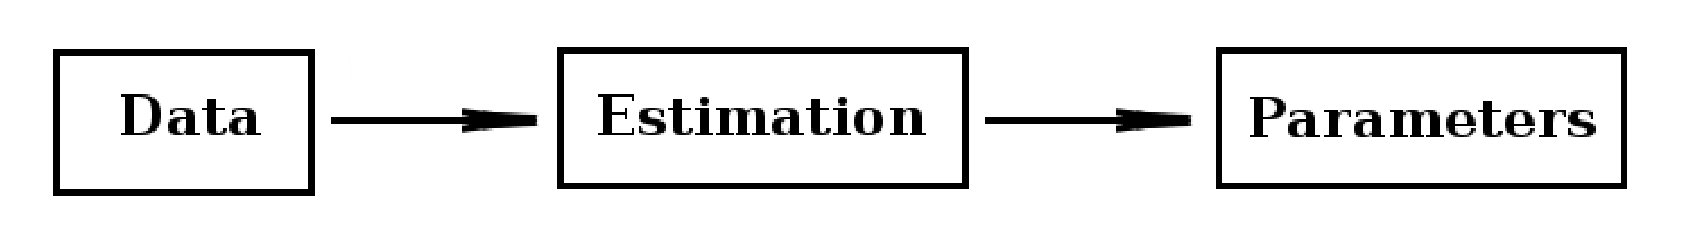
\includegraphics[width=\textwidth*\real{0.85}]{models2}
\end{center}

\caption{The input for the model in Figure \ref{modelflow} is the output for the estimation routine.}
\label{modelflowback}
\end{figure}


\comment{
As with many things in life, describing the process is much easier than
doing it.} The function box in Figure \ref{modelflow} is probably a
function in the mathematical sense, $f:\Xv, \betav \to \yv$. It may
be as simple as $\yv = \Xv\betav$ or an elaborate flowchart where
ingredients are mixed and re-mixed.  But as a practical matter, such
functions are really just pseudo-code, which we can make operational by
translating them into functions in the computational sense of a series
of instructions for a computer to follow.

I wrote this book to help you make that translation. The first focus
is purely mathematical: we need to select models and techniques bearing
in mind that they will eventually be code. The second focus is about
practical coding: your life is short, and you want to spend as little
of it as possible trying to coax systems into complying with your wishes
and learning yet more computer languages.

Fortunately, we have the technology. Before computers, we could only
use simple functions like linear combinations, because hunting for
parameters without a closed-form solution was impossible. 
But now that we can easily compute thousand-term likelihood functions
or take millions of random samples, we can use functions that mirror
reality better than a simple sum.

\comment{
The good news is that
doing math with a computer is unfettering. Instead of using restrictive
regression techniques designed before computers, we can use techniques
built around computing thousand-term likelihood functions, or taking
millions of random samples. These techniques originally appeared in
the textbooks as just theory, then eventually with a caveat that these
techniques are possible but computationally intensive. Now computations
are cheap, and we can use these techniques as we would their simplified
brethren.
}

In my own pain-filled experience, the best way to operationalize
statistical concepts is using C; the GNU Scientific Library,  which
facilitates the linear algebra and the Gaussian distribution work;
and SQLite, a package which facilitates handling large data sets. This
book will cover the basics of these components and the manner in which
we can translate from the mathematical language to the language these
libraries speak.  All of the tools and libraries
used in this book are open, in the sense that they may be freely
downloaded and used on the computer where you do your work right now.

The book also makes use of the Apophenia library, an open set of
functions based on the GSL and SQLite intended to simplify the hard
parts of using these packages for fitting models to data. Many books on
computing have a CD taped to the back cover providing useful code to
facilitate the methods used in the book; think of Apophenia as the code
appendix to this book.
\comment{
Most stats packages include a manual that attempts to instruct the reader,
and an alphabetical-order reference providing detailed usage notes for
functions and structures.  You are reading Apophenia's manual now,
and the reference is online at \url{http://apophenia.info/doc}.}

\paragraph{The goals}
Part I of this book will cover methods for efficient computing. Part II
is a catalog of models. Each model takes the
function box of Figure \ref{modelflow} to have a different form, and
then shows how to write the corresponding estimation function in Figure
\ref{modelflowback}. When listed by name, they are quite a long list; when
described via implementation in C, you will see that their estimation
involves the same set of simple techniques.  Part II also discusses
means of testing the parameters estimated using these methods.

Here is a more detailed list of the main topics covered:
\begin{itemize}
\itemsep 0pt
\item Structuring programs using modular functions and the stack of frames
\item Methods for reliability testing functions and making them more robust
\item Programming tools like the debugger and profiler
\item Databases: their utility, and how to get them to produce data in
the format you need
\item Probability: how famous distributions can be used to model data
\item Projections: summarizing many-dimensional data in two or three
dimensions
\item Estimating linear models
\item Methods of categorizing data and associating variables (aka data mining)
\item A brief review of classical hypothesis testing 
\item Writing models of the real world with an eye toward estimation and
hypothesis testing
\item Maximum likelihood estimation
\item Optimization routines: how they work and how to use them
\item Hypothesis testing using likelihood ratio tests
\item Monte Carlo methods for describing parameters
\item Bootstrapping and jackknifing for testing hypotheses
\end{itemize}

All of these things are independent of computing environment. However,
this book is about taking the computing part of computational modeling
and statistics seriously, so the concepts will be demonstrated both
in equation and flowchart form and in the form of executable code. As
noted above, the code will primarily be in C and SQL (Structured Query
Language).

This book falls in a mid-range between low-level numerical
computation and high-level use of prepackaged functions. For example,
{\sl Numerical Recipes in C} \citep{recipesinc} is a classic text
describing the algorithms for seeking optima and efficiently calculating
determinants. Being such a classic, there are many packages such as the
GSL that implement the algorithms from {\sl Numerical Recipes}, and this
book will build upon rather than replicate their effort. At the other
end, an abundance of texts will explain to readers how to do basic
statistics using the stats package of the month. This book lists the
one-line commands at this level, but it also breaks open the black boxes
and shows how those computations are done, so the reader can modify them
according to the vagaries of real-world data.

\paragraph{The intended audience}
I assume that you have had a statistics class or two already, and that
you have an encyclop\ae{}dic stats textbooks handy, so this book will
provide some utility as a statistics review, reference, or perhaps a
different perspective, but there are few proofs and no pretensions to
comprehensive coverage of classical probability and statistics.

If you are writing simulations, you will have interest in the chapters
on traditional statistics for a few reasons. First, 
the simpler the model, the better, and the classical statistical models
are as simple as they get. If one of those standard models fit your data well, you may not need to
draw out a more extensive simulation. Second, it is probably worthwhile to check
your data against a simple linear model as a baseline before going into
more complex waters. Finally, when you do run your simulation, you will
be marking down the variables in each period, thus producing a data set
that will need analysis, probably via classical statistical methods.

I assume that you are computer-literate, and have experience writing
scripts in a stats package. Those who are entirely new to the idea of
writing a sequence of instructions for a computer may want to warm up
with a few online tutorials.

If you are well-versed in C and SQL, then the later parts of Part I and
all of Part II will be immediately useful.
If you are not well-versed in C and SQL, then expect to take some time
getting comfortable with these languages before tackling the computational
implementation of the techniques discussed in Part II.

That is, there is an up-front investment to the methods here, and a
long-term payoff. If you expect that you will never do anything more
difficult than a linear regression on well-formed \ind{iid} data, or
if you are trying to slog through your department's stats requirement
so you can never look at another data set again, then by all means, put
this book down and get a copy of the easiest stats package you can
get away with. But if you expect to be doing computational modeling
and statistics for a larger part of your career, such that problems of
extensibility, portability, and scaling may be looming in your future,
then this book is for you.

It is not a short ride, but when you are done with all this---and this
is no exaggeration---you will have the tools to implement any technique
in classical statistics in existence today, on any data set, no matter
how large or exceptional.

\section{The programming covered}
\comment{
Using C is a mix of low-level and high-level
work. You will be allocating memory, telling the computer exactly where
to shunt its electrons. But, thanks to the efforts of tens of thousands
of programmers before you, you will have the benefit of functions that
will find the minimum of a function or calculate characteristics of a
Normal distribution, without having to remember Newton's method or
the equation for the Gaussian distribution.}

Part I is an overview of techniques for scientific computing: how to get
your computer to efficiently invert matrices and shunt large data sets.

It starts in Chapter \ref{c_crash} with a tutorial on the C programming
language.  The chapter covers nothing more difficult than adding
columns of numbers, but it provides the basic grammar and structure that
the remainder of the book will use to estimate models. Notably,
it introduces the idea of functions, and how one can build functions or
use existing functions to execute increasingly advanced routines.

\paragraph{Dealing with large data sets} Matrix-oriented packages,
(including the GSL) are not well-suited for data sets from agencies like
the US Census Bureau, that can be literally gigabytes of data.
C may seem unfriendly, but
those languages designed around dealing with large data sets tend
to be even more draconian---for example, SAS's data input command
is {\tt card}, referring to the punch card it expects you to put in the
hopper.\footnote{SAS, by the way, gets its facility with large data sets
by providing a front-end to SQL-like queries. You can enter SQL directly into
SAS if you so choose.}

Meanwhile, database systems are designed from the ground up to do nothing
but let you efficiently retrieve what you need from huge amounts of data.
But being so purpose-specific, databases do not provide a way to do
numerical analysis beyond taking averages.  Fortunately, we
are working in C, so we can have the best of all worlds. The technique
covered in this book (and the technique that Apophenia facilitates)
is to read all of your data into a database, and then query what you
need to a matrix, as you need it. This requires learning a new syntax,
\ind{SQL}, which is decidedly neither Beautiful nor Perfect, and adds a
level of complication on top of what you are already dealing with. But
the ease of manipulating data sets offered by SQL is very much worth
its short learning curve. Chapter \ref{sql} presents a tutorial of SQL
syntax to get you up to speed.

Apophenia implemenst SQL via the \ind{SQLite} library.
Those of you who 
have data which is already handled
by another database engine will easily be able to adapt the techniques
used here, but will need to brush up on the details of how to access
your site's database. Since you are using C,
you are guaranteed that there is an interface out there that you can
download and incorporate into your programs.

\paragraph{The computation engine} The \ind{GNU Scientific Library}
includes tools for all of the procedures commonly used in statistics,
such as linear algebra operations, looking up the value of F-, t-, $\chi^2$-
distributions, and finding maxima of likelihood functions. These
will be the building blocks for analysis. Chapter \ref{linear_algebra}
presents some basics for using the GSL, such as matrix manipulation and
linear algebra.

\paragraph{Apophenia}
Statistics textbooks could be much more brief. They could open
with notes on linear algebra and probability, and then conclude ``The
derivation of statistics from these basics is left as an exercise for
the reader.'' Similarly, the GSL includes all that we need to do
statistics, but in a raw form that is still a long way from the
sort of data analysis and hypothesis testing we want to do. Apophenia,
presented in Chapter \ref{apop}, is a library of structures and functions
that binds together the GSL and SQLite to facilitate the management of
data and models.

\paragraph{Pretty pictures} One thing C is not really good for is drawing
pretty pictures. This is not to be belittled, since those pictures
can be very persuasive. Consistent with the rest of this book, plotting
is done via \ind{Gnuplot}, a program which is freely available for
the computer you are using right now. Gnuplot is highly automatable, so once
you have a plot you like, you can have your C programs autogenerate
it or manipulate it in amusing ways, or can send your program to your
colleague in Madras and he will have no problem reproducing and modifying
your graphs. Once you have the basics down, animation and real-time
plots for simulations are easy. Chapter \ref{gnuplot} will cover creative uses of
Gnuplot to display data.


\input why_c.tex



\section{The stats covered} 
We can subdivide the goals of statistical analysis into two parts. The
first is to just say something interesting about a data set. This is often
model-free; for example, you may just want to show that two variables
are highly correlated, or that the data can mostly be summarized by three
dimensions.

The second part of statistical analysis is hypothesis testing, in which
we calculate a parameter of the data and then make a claim about that
parameter.  Having observed in the last paragraph that the correlation
coefficient of two variables is large, perhaps we would like to show
that that correlation coefficient is almost certainly different from
zero. More often, we have parameters in a model that we have written,
and would like to make claims about those parameters.

The techniques used for the two goals above are entirely different. For
example, there are any of a number of distributions listed in the
average stats textbook.  Poisson or Binomial distributions are used
only for describing data culled from the real world, while the Chi-squared
distribution or the F distribution are used only for testing hypotheses
about parameters we have written down ourselves (such as the correlation
coefficient, which has an F distribution). \citet[p 141]{kmenta} points out
that no notable natural population has a Chi-squared distribution.
\index{chi squared distribution@$\chi^2$ distribution}

Part II of this book will open with a chapter on describing data,
Chapter \ref{projections}, using simple calculations or projection
techniques. Chapter \ref{catchapter} will continue with other non-linear
means of describing and categorizing data. Then, Chapter \ref{gauss}
covers the hypothesis-testing half of the story, including methods of
comparing your data to various Gaussian distributions, such as the $t$
test, F test, and $\chi^2$ test, linear regressions, and goodness-of-fit
tests.



\paragraph{General theorems and their special cases}\index{Ordinary Least
Squares|(}
Here is another way to divide the theorems that underlie
statistics into two classes. The first class includes general
results about likelihood functions, that 
apply almost universally, but require a huge
amount of computational power to arrive at a result. The second class
consists of special cases of these general results, such as the theorems
underlying OLS regressions; these results impose more
assumptions, but are much easier to calculate, so that the results could
be used a century before computers were invented.\footnote{Historically,
the special cases came first and then were shown to be special cases of
more general results. Nonetheless, the rate of adoption of the general
cases has been in step with the speed of computing equipment.}


Have no doubt about it: the statistical methods we use are determined by
the technology we have at our disposal. Here is how a statistics textbook from 1939
\citep[p 43]{arkin:colton} explained how to use then-current technology to fit
a time trend:
\begin{quote}
To fit a trend by the freehand method draw a line through a graph of
the data in such a way as to describe what
appears to the eye to be the long period movement. \dots The drawing of
this line need not be strictly freehand but
may be accomplised with the aid of transparent straight edge or a
``French'' curve.
\end{quote}

A few decades ago, the special cases were the only class of results which
civilians had the computing power to use. This is when the stats packages
that are so prevalent today came to the fore, automating the tedium of
applying these special case results. The technology had an immediate
influence on how people did research: they applied those darn special
cases to everything, and one would have a hard time finding an issue of an
academic journal today that doesn't have at least one OLS regression.
Everything in the world has become a linear process.


\comment{
Using a projection technique instead of a less assumption-intensive and
more computation-intensive method is not quite as bad as just drawing a
line with a straightedge. But 

We spend most of our time in school learning the special cases,
because a few decades ago, this was the only class of results which
civilians had the computing power to use. This is when the stats packages
that are so prevalent today came to the fore, automating the tedium of
applying these special case results. The technology had an immediate
influence on how people did research: they applied those darn special
cases to everything, and one would have a hard time finding an issue of an
academic journal today that doesn't have at least one OLS regression.
Everything in the world has become a linear process.
}

The models in Part II are listed more-or-less in order of complexity.
The infinitely quotable Albert Einstein advised, ``make everything as
simple as possible, but not simpler.''  \index{Einstein, Albert}
The Central Limit Theorem tells us that errors often are
Normally distributed, and it is often the case that the dependent
variable is more-or-less a linear or log-linear function of several
variables. If such descriptions do no violence to the reality from
which the data was culled, then OLS is the method to use, and using more
general techniques will not be any more persuasive. 

But if the traditional statistical models are not appropriate, we now have
more at our disposal than a straightedge.
After the special cases are covered in Chapters \ref{projections}
and \ref{gauss}, Chapter \ref{mle} will show you how to write down the
likelihood functions to describe your model, as in Probit or Logit
estimations, how to find their maxima, and how to test hypotheses using
a likelihood ratio test.

Sometimes, even a likelihood function does not do justice to the model
you are attempting to describe, in which case the best thing to do is
simply write down the process, do a few million random draws from
that process, and see what properties those draws demonstrate.
Chapter \ref{boot} will cover Monte Carlo methods for such general
model description, including bootstrapping and jackknifing, which are
techniques to find variances from data when the classic Central Limit
Theorems fail.  

\comment{But it is no problem
if these assumptions are not true, because we have the computing power
to write down a model of the real world in arbitrary detail, and describe
and test that model in reasonable time.}  \index{Ordinary Least Squares|)}

\subsection{Typography}
Here are some notes on the conventions used throughout the book.

\exercise{Questions and exercises are marked like this paragraph.
The exercises are not thought experiments. It happens to all of us that
we think we understand something until we sit down to actually do it,
when a host of hairy details turn up. The exercises are 
relatively simple 
tasks that let you face the hairy details before your own real-world
complications enter the situation.}

\paragraph{\treesymbol Seeing the forest for the trees} Statistics textbooks
must tread a fine line. On the one hand, they must be didactic texts,
explaining concepts to the reader, while on the other they must be a
catalog of methods to apply should your data look just so.

Sections marked with a \ind{\treesymbol} cover details that may be
skipped on a first reading. They are not necessarily advanced
in the sense of being somehow more difficult than unmarked text, but a
reader who is trying to get the overall picture may want to cover them 
later. 

\paragraph{Some notation}  \hfill

$\Xv$: boldface, capital letters are matrices. All data matrices in this
book are organized so that the rows are each a single observation, and
each column is a variable.

$\xv$: lowercase boldface indicates a vector. Vectors are generally a
column of numbers, and their transpose, $\xv'$, is a row.

$\betav$: Greek letters indicate parameters to be estimated;
if boldface, they are a vector of parameters.

\ci{a} versus $a$: The teletype typeface indicates text
that can be typed directly into a text file and understood by C, SQL, or
the command prompt. Thus, when translating from a mathematical model
with variables $a$ and $b$, the typeface will shift to indicate the
analogous function inputs \ci{a} and \ci{b}.

\summarynoitems{Most sections end with a summary of the main points, set
like this paragraph.
Some readers will prefer to read the section summary at the end of
the section before reading the section itself.

The summary for the introduction:
\begin{itemize}
\item This book will discuss methods of estimating and testing the
parameters of a model with data.
\item It will also cover the means of writing those models using C, the
fastest, most stable, and most widely-available computing language in use today; and SQL, a 
language designed to help manage large data sets.
\end{itemize}
}


\comment{
\paragraph{Acknowledgments} Thanks to Ms. Annjeanette Agro for
graphic design suggestions.}








\comment{In case it is not obvious to you, we can not do statistical analysis without
computers.
In case it is not obvious to you, we can not do statistical analysis
without computers. 
But the mathematical explanation of a statistical procedure is
really just pseudo-code, which we can make operational by translating
it into real computer code. 
}

\comment{
As powerful as we like to think modern statistics is, it has a 
limited set of tricks at its disposal. For the purposes of this book,
I will divide them into three broad categories, which are broad enough
to cover the great majority of classical statistics (in fact, they overlap).

{\it Projections.} This includes the overused OLS linear regression (which is
a projection of your data onto a line), and the underused factor analysis
techniques. These are the techniques we humans use to reduce too many
dimensions down to something we can comprehend and even draw a picture of.

{\it Gaussian distribution tricks.} The Central Limit Theorem says that
a very wide range of statistics will have a Normal distribution. Square
the Normal, and we have a Chi-squared distribution. Take the ratio of two
Chi-squared distributions, and we have an F distribution.  The sum of
a random number of Normally distributed variables will have a Laplace
distribution.

{\it Likelihood function tricks.} Once we know the probability of an
event, probably thanks to a Gaussian distribution trick, we can then
write down the likelihood that a given set of parameters would bring
about the data we see, and then find the parameters that maximize this
likelihood. MLEs have the pleasing property of meeting the Cramer-Rao
lower bound, and the ratio of likelihood functions has the pleasant
property embodied in the Neyman-Pearson lemma, making them the basis of
hypotheses testing.

\subsection{The goals of statistics}
Let's settle an
important fact about statistical analysis: it proves nothing, only
persuades. A large part of this is that we are looking for causal stories
about the world, but there is no statistical technique (and never will be)
that proves \ind{causality}. Further, there is always a way to rewrite a model
or re-draw the data so that a rejected hypothesis is not rejected, or vice versa.
But some results are more robust to tweaking 
than others, and some models are just plain more persuasive than others.

Within the overall goal of persuasion, we}
\comment{
\section{Outline} 
Part I covers general scientific computing, and will be valuable to
anyone who needs to program a computer to handle and do math with large volumes of data.
Since I am assuming that you are computer-literate but
not a C programmer, Chapter \ref{c_crash} will give you a crash course
in C. It will not only get you familiar with the rules of the language,
but how to best think about problems in C. 
Chapter \ref{sql} will give you a quick overview of the second language,
SQL, which is a language that facilitates
producing tables of just the right form from a dataset. C and SQL are
excellent complements for data analysis: things which are very difficult
in one are often trivial in the other.
Chapter \ref{linear_algebra}
will then introduce you to the package of C functions most useful for
doing stats: the GNU Scientific Library (GSL). Notably, it will cover
how to do linear algebra using the GSL. Chapter \ref{apop} covers
Apophenia, a library of functions that bind together the GSL and SQLite
to facilitate data handling and statistics. Finally, Chapter
\ref{gnuplot} will cover creative uses of Gnuplot to display data.


Given those tools, coding statistics will be easy. Part II includes a chapter
devoted to each of the three categories of statistics above: Chapter \ref{projections}
handles the process of describing your data, using simple calculations
or projection techniques; Chapter
\ref{gauss} covers methods of comparing your data to various Gaussian
distributions, such as the t test, F test, and chi-squared test; Chapter
\ref{mle} will show you how to write down your likelihood functions and
find their maxima, as in Probit or Normit estimations, and how to test
hypotheses using a likelihood ratio test. Chapter \ref{boot} will cover
Monte Carlo methods such as 
bootstrapping and jackknifing, which are dirty tricks which will one
day save your life.  
}
